In this chapter we discuss the setup of the expiment from start to finish. My aim is to include as much detail as possible to eliminate all the experimental iterations I underwent in order to hone in on best process. \emph{I need to do some real thinking about the organization of this. Where do I want the derivation? Nathaniel had 2 chapters of introduction/background, then one for experimental setup, then data, then future stuff. I like that structure, but it feels weird, like I'm skirting around graphics and data until very late in the thesis.}


\section{Measuring Surface Stress via Adhesion}

\subsection{Force Balance Derivation}
When materials are soft or small enough, three main forces balance to determine the contact mechanics of the system. Adhesive forces increase the contact area between the silica sphere and the silicone substrate. Increasing the contact area has the effect of "pulling" the sphere into the gel. As a consequence, the substrate is being compressed [vertically], which is counteracted by the elastic forces within the bulk. This compression also has the effect of stretching the surface of the substrate, which is counteracted by substrate's surface tension. The force of gravity on the microsphere is negligible compared to the other forces. The density of silica (silicon-dioxide) is $2.65$ g/cm$^3$. For a very large sphere with radius (or is this diameter...) 50 microns, gravity applies a force of roughly 1.02e-08 N. \emph{I put the python script in die Diplomarbeit folder.}.

\subsubsection{Surface Energy}
$\Upsilon$ is the surface stress, which is equal to the energy cost per unit area required to create surface via cutting or stretching the material. For a flat substrate being stretched via the indendation of a sphere, the energetic cost is
\begin{equation}
\label{generic_surface_energy}
U_{surface} = \pi \Upsilon_{sv}\Delta A
\end{equation}

where $\Delta A$ is the change in surface area when stretched by part of an indenting sphere (spherical cap). Determining the change in area is a simple geometrical problem.

\begin{equation}
\Delta A = A_{cap} - A_{circle}. 
\end{equation}

Let a be the base radius of the circle projected on the plane of the substrate's surface. Let R be the radius of the indenting sphere, and d be the depth into which it is stretching. We can find a relationship between these variables using the Pythagorean theorem.

\begin{SCfigure}[][h]
	\begin{minipage}{.5\textwidth}
	\begin{align*}
	&a^2 + (R-d)^2 = R^2 \\
	&a^2 + R^2 - 2Rd +d^2 = R^2 \\
	&a^2 = 2Rd -d^2 \\
	&2Rd = a^2 + d^2
	\end{align*}
	\end{minipage}%
	\begin{minipage}{.5\textwidth}
	\centering
	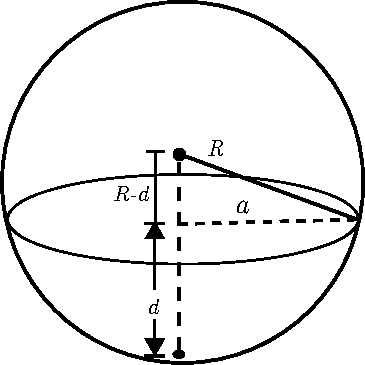
\includegraphics[width=.5\linewidth]{Chapters/Figures/SphericalCap}
	\caption{Spherical Cap Geometry}
	\label{fig:sphericalcap}
	\end{minipage}
\end{SCfigure}

%
%
%\begin{figure}[h]
%	\centering
%	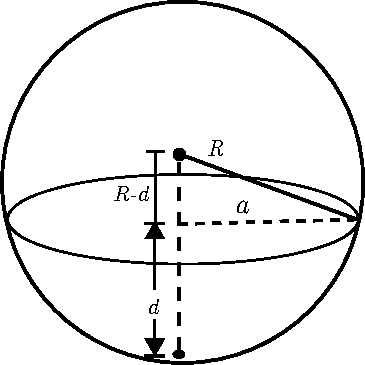
\includegraphics[width=.3\linewidth]{Chapters/Figures/SphericalCap}
%	\caption[Spherical Cap Geometry]{}
%	\label{fig:sphericalcap}
%\end{figure}
%
%\begin{align*}
%&a^2 + (R-d)^2 = R^2 \\
%&a^2 = 2Rd -d^2 
%\end{align*}
%

Now, solving for $ \Delta A $ and using the substituting the above relationship in the last step, we find

\begin{align*}
\Delta A &= 2\pi Rd - \pi a^2 \\
&= \pi(a^2+d^2) - \pi a^2 \\
&= \pi d^2
\end{align*}
 
 Rewriting (\ref{generic_surface_energy}), we can simplify surface energy in this geometry as 
 
 \begin{equation}
 \label{surface_energy}
 U_{surface} = \pi \Upsilon_{sv} d^2
 \end{equation}



\subsubsection{Elastic Energy}
The energy required to make a circular indentation of radius R and depth d is derived from Hertzian contact mechanics \cite{hertz1882uber}

\begin{equation}
\label{elastic_energy}
U_{elastic} \approx  \frac{ER^{1/2}d^{5/2}}{1-\nu^2}
\end{equation}
\emph{so I sort of read that German 1882 H. Hertz paper I just cited, and that equation doesn't show up. So I assume it's just derived from the contact mechanics Hertz laid down back then. Would like to better know where it comes from and derive it myself if room. Note, this equation was lifted from \cite{style2013surface}}.

This approximates a spherical cap in a flat plane.
\subsubsection{Adhesion Energy}
The energy of adhesion is W multiplied by the surface area in contact. Namely,
\begin{equation}
\label{W_energy}
U_{adhesion} \approx -2\pi W R d 
\end{equation}
where W is the adhesion energy. \emph{I think I should explain adhesion somewhere and talk about the Dupre equation 1869. Not sure where I want to put this, however. Maybe some of this stuff and the derivations should actually be in chapter 1}

\subsubsection{Force Balance}
At static equilibrium, the sum of the energies is:
\[U_{total} = \Upsilon_{sv} \pi d^2 + \frac{ER^{1/2}d^{5/2}}{1-\nu^2} - 2\pi W R d\] 
Because the energy balance is constant with respect to time, we can differentiate both sides, knowing that sum of forces is zero.

\begin{equation}
\label{THEeqn}
\frac{\partial U}{\partial t} = F = 2 \pi \Upsilon_{sv}d  + \frac{5cER^{1/2}d^{3/2}}{2 \left( 1-\nu ^2 \right) }  - 2 \pi WR = 0
\end{equation}


Eh, I should think about which part of the equation to put where. Should be the same order as the subsubsections above...Also, go look up what c is in the equation. dang I'm lazy.



\subsection{Gameplan .... change this subtitle. Suggestions?}
In equation \ref{THEeqn}, we can easily measure some of the parameters, and less easily measure others. The Young's Modulus, E, and the Poisson ratio, $\nu$ of the substrate can be measured separately for the substrate material. The depth $d$, and the radius $R$ of the sphere can be measured using fluorescent confocal microscopy. The only remaining terms, $W$ and $\Upsilon$, the adhesion energy and the surface stress, respectively, can be determined with a two-parameter fit. Alternatively, it is possible to measure the adhesion energy separately. This technique, though not critically important to the experiment, is of interest andf exploring if not just for the benefit of adding the capability to the lab.   

Of course, our interest is not just in developing a new technique for measuring, $W$ and $\Upsilon$, but in understanding how those values change when under strain. As needed, we have built our own equibiaxial stretching apparatus capable of maintaining up to 35\% strain in our silicone samples. The design is based off of previous work designed for stretching biological tissues \cite{na2008time} and is similar in design to the apparatus used in the 2017 $\Upsilon(\epsilon)$ measurements \cite{xu2017direct}. Design documents can be found in Appendix A, and an in-depth review of the stretcher can be found in Chapter 3. 

\subsection{The Process}
In the following section, I detail the steps needed in preparation for creating the measurements. My aim is to provide enough details that one could recreate my measurements, forgoing the trouble-shooting process I underwent. 

\subsubsection{Silcone Preparation and Spin Coating} 
In preparing our substrate, there are two important factors to consider: evenness of the surface and thickness. The substrate must be thick enough such that the the indenting microspheres do not feel a significant force from the thin PDMS underlayer. \emph{this probably sounds unclear. Change Later}. We know the stiffness of the gel we are curing, and by having a thick enough coating, we can ensure that the microspheres are only interacting with this gel. 100 $\mu m$ is a reasonable aim, and our substrates generally are between $80-100$ $\mu m$. The second concern is with thickness. In principal, as long as the surface is locally flat with respect to each microsphere, we can determine where the surface level lies and still measure the depth. In reality, it is not difficult to produce an even coating of silicone using a spin-coater. 

Before spin-coating it is useful to coat the underlayer with fluorescent beads. It is not vital, but this is helpful in determining the substrate's thickness. The only information obtained by this coating is the location of the substrate's bottom surface, so a dense bead coverage is not required, and could potentially be harmful if there is light bleeding. I suggest coating the bottom surface with 40nm beads for 1 minute. Full directions for preparing a fluroescent bead solution can be found in Appendix B. After this time, you may return the fluorescent beads back to the solution for re-use. A significant number of beads will remain on the underlayer. To remove some excess, gently wash the substrate with de-ionized water. For a coverslip, simply submerge the entire slip in water and gently remove it at a 45\degree angle, trying to prevent the water from breaking-up into smaller droplets. This process is slightly more difficult for the petri dish due to the larger size. I suggest  (either) using a very large container of water (it can be shallow, really you just need a large opening). If this proves challenging, I have found success using a 1000mL beaker tilted at an angle. It is also possible to use an autopipet for washing; repeat the same process used for the fluorescent bead coating, only use water this time. I have had mixed success with this technique, however. It often leaves a water droplet and has led to an uneven coating of fluorescent beads, manifested as streaks across the surface.

Depending on the silicone, a different amount of time should be waited before spin coating onto the desired surface. We coat our substrate onto glass for "zero applied strain" data or onto PDMS \emph{yeah I gotta look up the brand when I get back. I totally forget.} for stretching data. It is best that the silicone is far enough along in the curing process that it has enough stiffness and cohesiveness to remain on the underlayer when spun. As an extreme example, consider trying to spin-coat water; it would all fling off the underlayer. \emph{is there a better term than underlayer. I'm thinking of the general term for what we use a coverslip or stretchy circle}. For Gelest 9:1, there is no waiting time necessary; Gelest 9:1 cures rapidly. For Dow Corning 1:1, a wait time before spinning of 1 hour was observed. 

To help with the evenness of the coating, it is useful to degas the gel by leaving it in a vacuum chamber for a few minutes. A few small bubbles are not of concern, as the process of transferring the gel to the underlayer is enough to pop any remaining stragglers. I have found that a "glob" of gel roughly half the diameter of the underlayer, with the spin-coater set to 500rpm for 40sec is enough to create an even coating of roughly 100 $\mu m$.  

Coating a coverslip with silicone is a straightfoward process where hardly anything can go wrong. Coating the stretchable PDMS underlayer, however, requires some creativity to find the steps necessary to return the best results. I cut the PDMS disk with an X-acto knife and using a standard Petri \emph{2.5in diameter ...look up} dish as a template. In order to avoid snagging, I suggest cutting out the circle before removing the paper sheets on both sides of the silicone. Taping the Petri dish to the paper is also helpful prevent the dish from slipping while cutting. Unlike the glass coverslip, the PDMS underlayer is not rigid and must be place on a ridgid surface, such as a Petri dish, for spin coating. This leave the possibility that air bubbles could be trapped in between the PDMS and the Petri dish. This is a surefire way to ensure an uneven and frustrating substrate. I suggest removing the top paper sheet of the newly cut PDMS, then placing the Petri dish down upon the exposed silicone. You should now have a Petri dish with a silicone disk on top and a paper sheet on top of that. Using your thumbs, simply do your best to push all the air bubbles from the center outwards. Finally, any tiny air bubbles can hopefully be removed by placing the Petri dish in a vacuum chamber for a few minutes. Now you can coat the PDMS with fluorescent beads and wash as desired before place the petri dish onto the spin-coater and proceeding as described above.

After spin-coating, the silicone requires time to cure. We cure Dow-Corning 1:1 for at room temperature for at least 24 hours. For Gelest 9:1, we oven cure at $70 \degree$ C for at least 24 hours. Either silicone can be cured at room temperature or in the oven so long as a sufficient amount of time is waited, however, we have used this methods to maintain consistency, as well as parallel the techniques used in previous literature \cite{xu2017direct}.

After the silicone cures, it is time to coat the surface with fluorescent beads again. It is important that the beads are dense enough to give a high resolution, yet not so dense as to become indistinguishable; this presents a challenge the MATLAB particle locating software. Secondly, too dense a bead coverage risks light bleeding to vertically adjacent stacks. For the 40nm bead solution prescribed in Appendix B, I suggest letting the solution soak for up to 3 minutes before removing and washing the substrate. While the fluorescent beads chosen are most susceptible to light at \emph{shoot, what wavelength? Like 440?} nm, there is still the risk of photobleaching the fluorophores, and worth dimming the lights in the lab when working with them. 

The final preparation step is to sprinkle silica spheres of a range in size on top of the silicone. This should be done at least 30 minutes before collecting data so that the spheres have time to settle into an equilibrium state into the silicone. From a side view, the final setup should look as follows:



\subsubsection{Fluorescent Confocal Microscopy}
Data was obtained using the Nikon Ti2 Eclipse Microscope as the base, attached to the A2 Confocal \emph{right? The naming has always been confusing}. To take image stacks of the Fluorescent beads, we use a 50x water-immersion objective lens. We set the laser to 440nm and adjust the power (HV) and gain as needed. Generally these values are around 5.0 and 40 respectively. \emph{so, does this mean anything to anyone but me? Like, I don't even know what units that would be, and I doubt it translates to anything other than the Nikon machines, right?} In order to get clear locating, it is important not to saturate the photo-detector. 

\begin{figure}
	\centering
	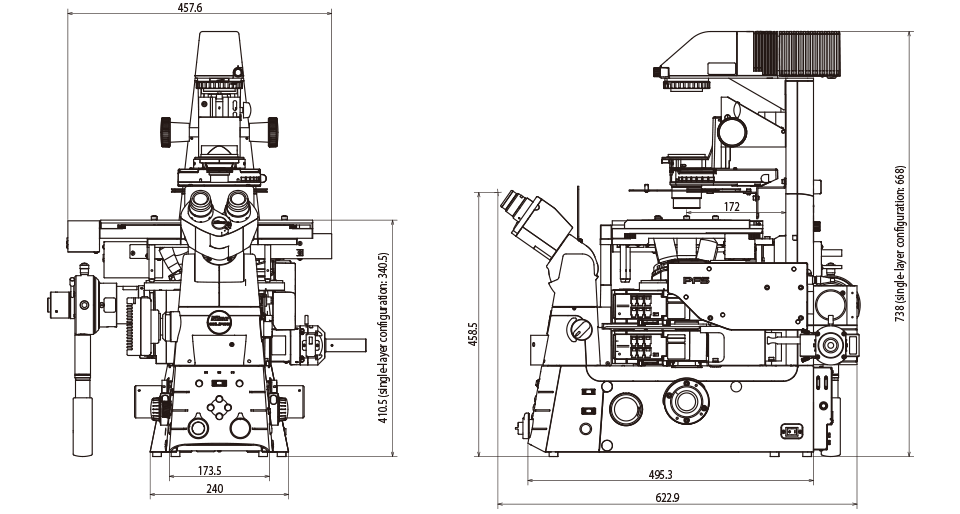
\includegraphics[width=0.7\linewidth]{confocal_stuff/Ti2_diagram_1}
		\caption[Nikon Ti2 Microscope Base]{This may only be here because it's pretty....Also, I'd like to remove the measurements when I have time. Also, not sure how to cite the manual yet.}
	\label{fig:ti2diagram1}
\end{figure}

For silica spheres ranging from $5-50 \mu$m in size, we have found the best scaling factor to be $.104 \mu$m/pixel in the horizontal plane for an image of 1024 x 1024 resolution. We set the vertical step size (z-direction) to $.225 \mu$m/px or $.25 \mu$m/px depending on what the confocal recommended. Both provided adequate vertical resolutions. 16x averaging using the resonant scanner took up to 5 minutes per scan, but provided excellent resolution. 


\section{Stretch Calibration}
\emph{So I have a section in chapter 3 about this. I'm starting to think that maybe it shouldn't be there, and I should just go in depth about it here. But then chapter 3 is going to be super short, and maybe I should just turn it into an appendix. For now, I'm going to write about it in chapter 3 as I would if it were to be here, then decide later where I'd rather put it.} So.... See chapter 3
